%-------------------------------------------------------------------------------
% File: main.tex
%       StockSim project documentation.
%
%       Compile using:
%           $ pdflatex main.tex
%
% Author: Marco Pinna <>
%         Rambod Rahmani <rambodrahmani@autistici.org>
%         Yuri Mazzuoli <>
%         Created on 05/11/2020
%-------------------------------------------------------------------------------
\documentclass[11pt, a4paper, twoside, openright]{book}

% equal left and right margins
\usepackage[hmarginratio=1:1]{geometry}

% configuration to typeset documents in italian
\usepackage[english]{babel}

% include graphics in the file
\usepackage{graphicx}

% used in the dedication environment definition
\usepackage{afterpage}

% used to set page background image
\usepackage{tikz}

% url and hyper links setup
\usepackage{hyperref}
\hypersetup{
    colorlinks=true,
    linkcolor=black,
    filecolor=magenta,      
    urlcolor=blue,
}

\let\cleardoublepage=\clearpage

% blank page command
\newcommand{\blankpage}
{
    \null
    \thispagestyle{empty}%
    \addtocounter{page}{-1}%
    \newpage
}

% dedication environment
\newenvironment{dedication}
{
    % blank page before dedication
    \afterpage{\blankpage}
    % we want a new page
    \clearpage
    % no header and footer
    \thispagestyle{empty}
    % some space at the top
    \vspace*{\stretch{1}}
    % the text is in italics
    \itshape
    % flush to the right margin
    \raggedleft
    % blank page after dedication
    \afterpage{\blankpage}
}
{
    % end the paragraph
    \par
    % space at bottom is one times that at the top
    \vspace{\stretch{1}}
    % finish off the page
    \clearpage
}

\usepackage{color}

\definecolor{pblue}{rgb}{0.13,0.13,1}
\definecolor{pgreen}{rgb}{0,0.5,0}
\definecolor{pred}{rgb}{0.9,0,0}
\definecolor{pgrey}{rgb}{0.46,0.45,0.48}

% Java listings settings
\usepackage{listings}
\lstset{language=Java,
  showspaces=false,
  showtabs=false,
  breaklines=true,
  showstringspaces=false,
  breakatwhitespace=true,
  commentstyle=\color{pgreen},
  keywordstyle=\color{pblue},
  stringstyle=\color{pred},
  basicstyle=\ttfamily,
  moredelim=[il][\textcolor{pgrey}]{$$},
  moredelim=[is][\textcolor{pgrey}]{\%\%}{\%\%}
}

\definecolor{dkgreen}{rgb}{0,0.6,0}
\definecolor{gray}{rgb}{0.5,0.5,0.5}
\definecolor{mauve}{rgb}{0.58,0,0.82}
\definecolor{gray}{rgb}{0.4,0.4,0.4}
\definecolor{darkblue}{rgb}{0.0,0.0,0.6}
\definecolor{lightblue}{rgb}{0.0,0.0,0.9}
\definecolor{cyan}{rgb}{0.0,0.6,0.6}
\definecolor{darkred}{rgb}{0.6,0.0,0.0}

\lstset{
  basicstyle=\ttfamily\footnotesize,
  columns=fullflexible,
  showstringspaces=false,
  numbers=left,                   % where to put the line-numbers
  numberstyle=\tiny\color{gray},  % the style that is used for the line-numbers
  stepnumber=1,
  numbersep=5pt,                  % how far the line-numbers are from the code
  backgroundcolor=\color{white},      % choose the background color. You must add \usepackage{color}
  showspaces=false,               % show spaces adding particular underscores
  showstringspaces=false,         % underline spaces within strings
  showtabs=false,                 % show tabs within strings adding particular underscores
  frame=none,                   % adds a frame around the code
  rulecolor=\color{black},        % if not set, the frame-color may be changed on line-breaks within not-black text (e.g. commens (green here))
  tabsize=2,                      % sets default tabsize to 2 spaces
  captionpos=b,                   % sets the caption-position to bottom
  breaklines=true,                % sets automatic line breaking
  breakatwhitespace=false,        % sets if automatic breaks should only happen at whitespace
  title=\lstname,                 % show the filename of files included with \lstinputlisting;
                                  % also try caption instead of title  
  commentstyle=\color{gray}\upshape
}

\lstdefinelanguage{XML}
{
  morestring=[s][\color{mauve}]{"}{"},
  morestring=[s][\color{black}]{>}{<},
  morecomment=[s]{<?}{?>},
  morecomment=[s][\color{dkgreen}]{<!--}{-->},
  stringstyle=\color{black},
  identifierstyle=\color{lightblue},
  keywordstyle=\color{red},
  morekeywords={xmlns,xsi,noNamespaceSchemaLocation,type,id,x,y,source,target,version,tool,transRef,roleRef,objective,eventually}% list your attributes here
}

\usepackage{dirtree}

%-------------------------------------------------------------------------------
% Title page
%-------------------------------------------------------------------------------
\title{
    \vspace{-3cm}
    \includegraphics[scale=0.3]{img/cherubino_black.eps}\\
    {\scshape University of Pisa}\\
    School of Engineering\\
    \rule{7cm}{0.01cm}\\
    {\normalsize{\scshape Large Scale and Multi-Structured Databases}}\\
    [2cm]
    {\scshape StockSim: Stock Portfolio Simulator}\\
    [3cm]
    \LARGE{\textbf{Supervisor}\hfill\textbf{Students}}\\
    \Large{\emph{Prof. Pietro Ducange}\hfill\emph{Marco Pinna\\}}
    \Large{\hfill\emph{Rambod Rahmani\\}}
    \Large{\hfill\emph{Yuri Mazzuoli\\}}
    \vfill
    \date{\today}
}

% leave the author field ampty in the title page
\author{}

%-------------------------------------------------------------------------------
% Document beginning
%-------------------------------------------------------------------------------
\begin{document}

% make title page
\maketitle

% blank page before dedication
\afterpage{\blankpage}	

% enable page numbering back: roman numbers style
\pagenumbering{roman}

% print table of contents
\tableofcontents

% set arabic page numbering style
\pagenumbering{arabic}

%-------------------------------------------------------------------------------
% Part I: Documentation
%-------------------------------------------------------------------------------
\part{Documentation}
%-------------------------------------------------------------------------------
% File: introduction.tex
%       Part of StockSim project documentation.
%       See main.tex for further information.
%-------------------------------------------------------------------------------
\chapter{Introduction}
{\Large StockSim} is a Java application which allows users to simulate stock portfolios.
It uses statistical models built from U.S. stock market stocks and ETFs historical data day by day, starting from YEAR.

%-------------------------------------------------------------------------------
% File: requirements.tex
%       Part of StockSim project documentation.
%       See main.tex for further information.
%-------------------------------------------------------------------------------
\chapter{Actors and requirements}
The main actors and the functional requirements can be defined using the simple
application description provided in the introductory chapter. Non-functional
requirements, described in detail in the second section of this chapter, are the
characteristics that ensure satisfactory interaction with users and real world
utility of the product.

\section{Actors}
Based on the application design, four main actors can be identified:
\begin{itemize}
    \item A \textbf{Guest user} is someone who is not yet registered (does not
    have a valid account to be able to use the application); this actor does not
    own private credentials for the login; in order to exploit the application
    main functionalities, he must register a new user account; therefore, the
    registration is the only action allowed for a Guest;

    \item A \textbf{Registered user} is someone who sign up on the application;
    this actor owns private credentials (username and password) for the login;
    he can login as a user into the client application and utilize its main
    features to watch stocks information, compose portfolios and simulate them. 
   
    \item An \textbf{Admin user} is someone who is registered on the application
    with administration credentials; this actor can login as an admin into the
    client to perform maintenance operations; these operations include, among
    others, checking the integrity of the entire database and add new stocks to
    it;

    \item The \textbf{Data Updater} is a thread running on StockSim Server; this 
    thread is supposed to be always running, and it is in charge of updating the
    database historical data with the new information coming from the stock
    market daily trading sessions; it is also in charge of finding and fixing
    (or at least report) integrity issues.
\end{itemize}
Please refer to Chapter 3 for the full use case diagram.

\section{Requirements}

\subsection{Functional requirements}
\begin{itemize}
	\item The user, upon launching the application, should be able to sign-up and sign-in.
	\item The user should be able to search for a stock and view related details.
	\item The user should be able to view charts of the historical data of a stock.
	\item The user should be able to create and delete portfolios.
	\item The user should be able to add/remove stocks to/from their portfolio.
	\item The user should be able to run simulations on a portfolio.
	\item The user should be able to visualize statistics about a simulation and possibly view related charts.
	\item Only admins should be able to add new stocks to the database.
	\item Only admins should be able to create new admin accounts.
	\item Only admins should be able to delete admin accounts.
	\item Only admins should be able to delete user accounts.
	\item The software should always provide the most recent data available for a stock.
\end{itemize}

\subsection{Non-functional requirements}
\begin{itemize}
	\item The retrieval of data about stocks and portfolios should be fast.
	\item User password should be stored in a secure way (i.e. hashed).
\end{itemize}

%-------------------------------------------------------------------------------
% File: UML_diagrams.tex
%       Part of StockSim project documentation.
%       See main.tex for further information.
%-------------------------------------------------------------------------------
\newgeometry{bottom=0.1cm}
\chapter{UML diagrams}
\section{Use Case diagram}
\begin{figure}[H]
	\begin{center}
		\includegraphics[scale=0.22]{img/use_case.jpg}
	\end{center}
\end{figure}
\restoregeometry
\section{Class diagram}
\includegraphics[scale=0.20]{img/design_class_diagram_duc.png}

%-------------------------------------------------------------------------------
% File: database.tex
%       Part of StockSim project documentation.
%       See main.tex for further information.
%-------------------------------------------------------------------------------
\chapter{Database}
The database is composed by 8236 stocks from the US stock market, along with
their general information and historical data; the application also needs to
store users and admins login credentials, personal information and the
composition and details of each user's portfolio.
We decided to use a column database (Apache Cassandra) for the storage of
historical data; this is because historical data represents almost the 99\%\ of
the entire database and is going to be growing very fast as days go by;
aggregation and financial analytics on these volumes of data will perform better
in a column database where data storage is designed to optimize this type of
operations by column.\\
We decided to store any other information using a document database (MongoDB),
in order to exploit the schemaless property to save memory; data frequently
needed together is stored in the same document and indexes were created to speed
up linking between documents; 

\section{Dataset}
The initial set of data was fetched from the web: using Python scripts with
\texttt{pandas}, \texttt{yfinance} and \texttt{JSON} as support libraries and
relaying upon \url{www.nasdaqtrader.com} and \url{finance.yahoo.com}.
\subsection{NasdaqTrader}
The Nasdaq Stock Market (Nasdaq) is the largest U.S. equities exchange venue by volume. 
https://www.nasdaqtrader.com/ \\
We choose to take our set of stocks from the Nasdaq index, because it is very popular and
include a large number of stock, representative of different economy sector. This will allow 
users to interact with big and famous companies stocks (like Google, Apple, Tesla...), but also
to try smaller companies and/or minor sectors investments. 
NasdaqTrader provides us a stock symbols' list of all the stocks entered in the NASDAQ index
from 1970 until now;
\subsection{Yahoo! Finance}
"Yahoo Finance provides free stock quotes, up-to-date news, portfolio management resources, 
international market data, social interaction and mortgage rates that help you manage your 
financial life." https://finance.yahoo.com/ \\
Yahoo Finance is a service, been part of the Yahoo network, that provides a lot of information
about stocks and companies; they are frequently updated, reliable and well organized.\\
We decided to use this service to retrieve the starting dataset of stocks; we extract only 
the fields that we needed, and parse into a JSON file. In this way 
is possible to rebuild from scratch this dataset into MongoDB with few commands (including
mongoimport).
With Yahoo Finance is also possible to retrieve historical data of market values for every 
stocks. Using this service it has been possible to build a dataset of all the market values of
each stocks coming from NasdaqTrader; values are collected daily, and we decided to take all 
the values from 2010 to 2020; this dataset (around 1.43 GB) has been parsed to CVS files and
than imported into a Cassandra Cluster. Thanks to the Yahoo Finance service, it's possible
to update every day the database with the last session results. It's also possible to add a new
stock to the dataset, coming from every market exchange of every country.\\
\includegraphics[scale=0.12]{img/dataset_comp.png}\\


\section{MongoDB}
"MongoDB is a general purpose, document-based, distributed database build
for modern application developers and for the cloud era." Taken from www.mongodb.com.\\
MongoDB is a very famous document database with a great support for cloud operations, which 
will improve the availability of our application. It also supports several analytic functions
and the creation of custom indexes in order to speedup read operations.
In order to organize data in a meaningful and memory-optimal way, we opted for this structure:

\includegraphics[scale=0.17]{img/mongoDB_schema.png}\\

This scheme is composed by 3 collections: \textbf{stocks}, \textbf{users}, \textbf{admins};
\begin{itemize}
    \item
The stocks collection contains one document for each stock; inside this document are stored 
all the general information about the stock, which is identified by the attribute SYMBOL;
some basic information are always present, while others are missing for some stocks; we decided 
to keep these last type of information where possible, exploiting the schemaless property of
the document database;
    \item
The \textbf{users} collection contains one document for each user registered on the application; for every
user login credentials are stored, along with few personal information; for every user is 
also stored an array of documents named PORTFOLIOS: this array contains the portfolios of the user.
Each portfolio has a scheme, witch include an array of TITLEs, named COMPOSITION, witch represent
the settlement of the portfolio itself. This nested structure has been preferred over splitting
data in different collections, because all the information of a user, including their portfolios, 
are frequently needed together; on the other hand, there are not operations that involve
portfolios owned by different users.
    \item 
The \textbf{admins} collection contains the admins login credentials together with few personal
informations about them; we decided to create a separated collection for administrators 
to improve the security of the administration features: in this way is impossible to inject
administration privileges through the login command.
\end{itemize}
\subsection{Aggregations}
One of the main features of our application is the possibility to choose some stocks from
the market and combine them into a portfolio. When a user is looking for a stock, they want to
know statistic about \textbf{industries} and \textbf{sectors}, along with classification by 
\textbf{level of capitalization} and  \textbf{PE ratio}; in order to do so, we will provide
these aggregation pipelines:
\begin{itemize}
    \item the total market capitalization of each sector
    \item the total market capitalization of each industry
    \item the total market capitalization of stocks coming from the same country
    \item the average PE ratio of stocks working in the same sector
    \item the average PE ratio of stocks working in the same industry
    \item the average PE ratio of stocks coming from the same country
    \item the average PE ratio of stocks being in a specific range of market capitalization
\end{itemize}
We provide here an example of an aggregation Mongo query:
\begin{lstlisting}[basicstyle=\footnotesize,language=Java,numbers=left,
    numberstyle=\footnotesize,numbersep=4pt,frame=single]
    /**
    * Aggregates data with filtering and grouping by an attribute, can compute
    * sum, avg ecc.
    *
    * @param collection the collection where to perform the operation;
    * @param filter filter to be used to find the documents.
    * @param groupField the filed used to group the aggregation
    * @param aggregator the aggregator function and field
    *
    * @return iterable object containing the result of the aggregation.
    */
   public AggregateIterable<Document> aggregate(final Bson filter, final String groupField, final BsonField aggregator, final MongoCollection<Document> collection) {
       Bson match = Aggregates.match(filter);
       return  collection.aggregate(
               Arrays.asList(match, Aggregates.group("$"+groupField, aggregator)));
   }
\end{lstlisting}
\begin{lstlisting}[basicstyle=\footnotesize,language=Java,numbers=left,
    numberstyle=\footnotesize,numbersep=4pt,frame=single]
    MongoCollection<Document> collection1 = 
        dbManager.getCollection(
            StocksimCollection.STOCKS.getCollectionName()
        );
    // aggregate examples
    final Bson equity= eq("quoteType", "EQUITY"); //filter(s)
    // name of the field projected, field to accumulate
    // type of accumulation (sum, avg...)
    final BsonField marketCapAccumulator=Accumulators.sum("totalCap","$marketCap");
    AggregateIterable<Document> aggregateList =
                                        // grouping attribute
            dbManager.aggregate(equity, "sector", marketCapAccumulator, collection1);
    for (Document document : aggregateList) {
        System.out.println(document);
    }
    // avg example with nested attribute
    final BsonField PEAccumulator=Accumulators.avg("avgPE","$trailingPE");
    aggregateList =
            dbManager.aggregate(equity, "location.country",
                    PEAccumulator, collection1);
    for (Document document : aggregateList) {
        System.out.println(document);
    }
\end{lstlisting}
\subsection{Indexes}
In order to speeup read operation in the document database, 
we decided to introduce some custom indexes:
\begin{itemize}
    \item a REGULAR and UNIQUE index on the attribute \textbf{symbol} in the collection stocks;
    \item a REGULAR index on the attribute \textbf{marketCAP} in the collection stocks;
    \item a REGULAR index on the attribute \textbf{trailingPE} in the collection stocks;
    \item a REGULAR index on the attribute \textbf{sector} in the collection stocks;
    \item a REGULAR index on the attribute \textbf{industry} in the collection stocks;
    \item a REGULAR index on the attribute \textbf{country} in the collection stocks;
    \item a REGULAR and UNIQUE index on the attribute \textbf{username} in the collection users;
\end{itemize}
We provide some statistic that endorse our idexes choises\\

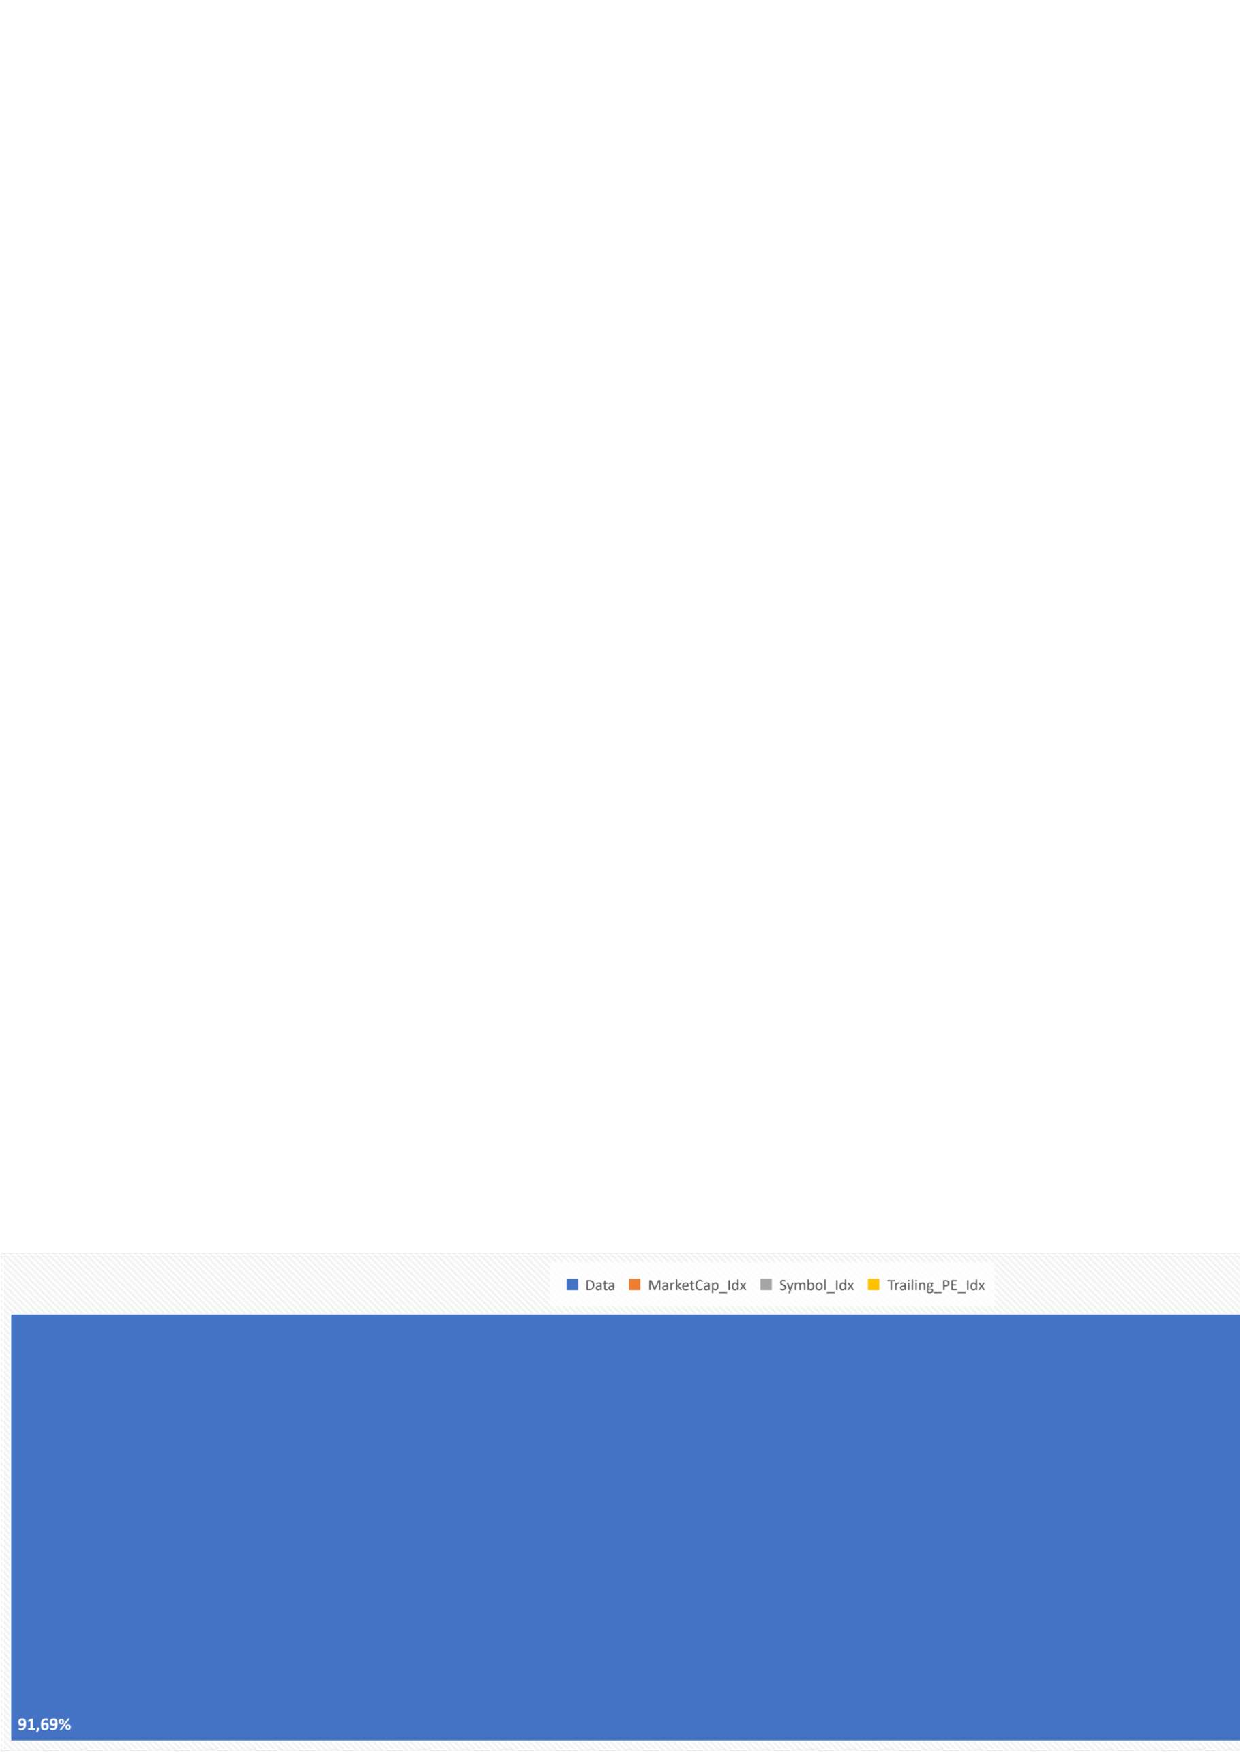
\includegraphics[scale=0.11]{img/memory_mongo.png}
\includegraphics[scale=0.11]{img/latency_mongo.png}\\

Analog results can be found about the username index in the users collection.

\section{Apache Cassandra}
"The Apache Cassandra database is the right choice when you need scalability and high 
availability without compromising performance. Linear scalability and proven fault-tolerance 
on commodity hardware or cloud infrastructure make it the perfect platform for mission-critical 
data. Cassandra's support for replicating across multiple datacenters is best-in-class, 
providing lower latency for your users and the peace of mind of knowing that you can survive
regional outages." www.cassandra.apache.org\\
Apache Cassandra is a database designed for high scalability and availability; it's 
capable to handle a huge amount of data and manage it in a decentralized architecture
across multiple nodes. It's build to be write optimized, but with right indexes choices
also read latency can be improved; tables schemes and analytic functions can be customized.
This is the scheme of our Cassandra database:\\
\includegraphics[scale=0.2]{img/cassandraDB_scheme.png}\\

\subsection{Aggregations}
In order to provide snapshots and statistics of stocks and portfolios trends over time,
we exploit the customization functionalities of Cassandra; a custom aggregation has been 
created, specifically to provide aggregate values of more than one day, for a given
period of time; this allows us to obtain different granularity for stock market data,
computed on server side; this will not over overwhelm the server, because the aggregator will
execute, for each row, between a memory access and the following. This will greatly reduce
the data to be transmitted from the node to the client, saving bandwidth and time.  \\

\begin{lstlisting}[basicstyle=\footnotesize,language=SQL,numbers=left,
    numberstyle=\footnotesize,numbersep=4pt,frame=single]

    /* State function to be executed for every row*/
    CREATE OR REPLACE FUNCTION PeriodStateParam ( 

    /* the state, containing the aggregation result till this row */
        state map<date,frozen<map<text, float>>>,
    /*  the parameter ndays indicate the duration 
    *   of the period aggregation, in days          */
        ndays int, data date,  
        open float,  close float , high float,  low float, 
        volume float ,  adj_close float)
    CALLED ON NULL INPUT 
    RETURNS map<date,frozen<map<text, float>>> 
    LANGUAGE java AS '
    if (data != null) { 
        int d=0;
        Map<String, Float> statemap=null;
       
        for(d=1; d<ndays;){
            if((statemap=state.get(
                    data.add(Calendar.DAY_OF_MONTH,d)
                ))!=null)
                break;
            d++;
        }
        if(d==ndays){
            statemap=new HashMap<String, Float>();
            statemap.put("open", open);
            statemap.put("close", close);
            statemap.put("high", high);
            statemap.put("low", low);
            statemap.put("volume", volume);
            statemap.put("adj_close", adj_close);
            state.put(data,statemap);
        }
        else{
                if(high>statemap.get("high"))
                    statemap.replace("high", high);
                if(low<statemap.get("low"))
                    statemap.replace("low", low); 
                statemap.replace("volume",statemap.get("volume")+ volume);
                statemap.replace("open",open);
                state.replace(data, statemap); 
        }
    } 
    return state;'
     ;
    
    /*  aggregate declartation
    *   this aggregation geenrate a map data structure (JSON like):
    *   the key is the end date of each period of nday days, 
    *   and the value is another map containing the aggregate 
    *   values of the period as:
    *        the open of the first day
    *        the close and adjusted close of the last day
    *        the maximun of the highs
    *        the minimum of the lows
    *        the sum of the volumes
    */
    CREATE OR REPLACE AGGREGATE PeriodParam 
        ( int, date,float, float,float, float,float, float ) 
    SFUNC PeriodStateParam
    STYPE map<date,frozen<map<text, float>>>
    INITCOND {}; /* no initial condition is necessary */
    
    /* example of usage, it can be used also with grouping by symbol */
    select PeriodParam(
        20, date, open, close, high, low, volume, adj_close)
        as Period from tickers where 
        date<'2020-12-1' and date>'2020-6-10' 
        and symbol='TSLA';
    
\end{lstlisting}

\subsection{Indexes}
\begin{itemize}
    \item 
The PARTITION KEY index is part of the PRIMARY KEY and it is used to shard the dataset across
the nodes. This index is build on the string symbol, unique for each stock;
    \item
the CLUSTERING KEY i is also part of the PRIMARY KEY, and it's used to maintain rows 
chronological order. This index is build on the attribute date;
\end{itemize}
\section{Sharding and Replicas}
The MongoDB cluster and the Cassandra cluster are deployed on 3 virtual machines provided
by the University of Pisa; 
Our architecture is oriented to the availability of the service, and build for the maximum
scalability and decentralization.
\begin{itemize}
    \item 
The Cassandra cluster is build among all 3 nodes, and data are sharded by the ticker symbol;
in this way every node store 1/3 of the main dataset, and aggregation functions are computed
on records that stay in the same node; each node also stores a backup of the data
assigned to another node, giving us a replication factor of 2. There are 2 seed nodes,
which are responsible for the cluster: the cluster is online as long as one of them keeps
working. This is indeed a minor issue, because in any case, with only one node, the dataset 
would by incomplete. The decentralized behaviour of Cassandra ensures that
even if all the node were to go offline, the cluster would return available as soon as one seed server went back
online. 
    \item
The MongoDB cluster is also build among all 3 virtual machines, and the service is replicated;
an initial primary server is elected, then another one will take it's place if it goes down. 
The cluster is available as long as one server is working, and incoming traffic could be balanced
with the "nearest" preference on client connection; in this way the client would connect to the
server with the lowest ping time.

\end{itemize}
\includegraphics[scale=0.2]{img/cluster_diagram.png}\\
\section{Apache Cassandra vs MongoDB}

%-------------------------------------------------------------------------------
% File: software_architecture.tex
%       Part of StockSim project documentation.
%       See main.tex for further information.
%-------------------------------------------------------------------------------
\chapter{Software architecture}

%-------------------------------------------------------------------------------
% File: conclusions.tex
%       Part of StockSim project documentation.
%       See main.tex for further information.
%-------------------------------------------------------------------------------
\chapter{Conclusions}
The modular architecture of the project (Chapter 5) allowed us to create
stand-alone APIs (for both the databases and Yahoo Finance) that are not
inherently tied with the StockSim application or with financial applications in
general. They all can possibly be used stand-alone and could be integrated in
different projects.\\
\\
Most of the choices we made during both the designing and the development
process proved to be effective. We opted for a column database architecture to
store the historical data because it really lends itself to such usages.
Performance analysis of the query latency (as shown in paragraph 4.5) confirmed
our hypothesis, although tests have been run only locally.\\
It would be interesting to repeat the measurements with a bigger database and in
a controlled environment where network jittering does not skew the results too
much, something that we were not able to do due to limited resources of the VMs
and due to the fact that all traffic is filtered through a VPN.\\
\\
At the moment the database is limited to the US market data only, but it would
be really simple to integrate data from other stock markets around the world
using the StockSim Client in \texttt{admin} mode.\\
From the Software and Data Model architectural point of view, this would not be
a problem since the column database architecture is by nature suitable for
geographical distribution and for dealing with huge amounts of data. Another
test worth doing to evaluate the performance of the application would be to
deploy several geographically distributed servers and increase the data volume
by some orders of magnitude: the current database size is around 1.43 GB and it
would be interesting to see how it behaves with tens of terabytes of data.

%-------------------------------------------------------------------------------
% File: appendices.tex
%       Part of StockSim project documentation.
%       See main.tex for further information.
%-------------------------------------------------------------------------------
\chapter{Appendices}

\chapter*{Appendix A}
%TODO reduce spacing before chapter title so that first pom is not broken in 3 pages but only in 2.

\lstinputlisting[basicstyle=\footnotesize,language=XML,numbers=left,
numberstyle=\footnotesize,numbersep=8pt,frame=single]{pom_files/parent_pom.xml}

\lstinputlisting[basicstyle=\footnotesize,language=XML,numbers=left,
numberstyle=\footnotesize,numbersep=8pt,frame=single]{pom_files/client_pom.xml}

\lstinputlisting[basicstyle=\footnotesize,language=XML,numbers=left,
numberstyle=\footnotesize,numbersep=8pt,frame=single]{pom_files/server_pom.xml}

\lstinputlisting[basicstyle=\footnotesize,language=XML,numbers=left,
numberstyle=\footnotesize,numbersep=8pt,frame=single]{pom_files/library_pom.xml}

%-------------------------------------------------------------------------------
% Part I: User Manual
%-------------------------------------------------------------------------------
\part{User Manual}
%-------------------------------------------------------------------------------
% File: user_manual_CH1.tex
%       Part of StockSim project documentation.
%       See main.tex for further information.
%-------------------------------------------------------------------------------
\chapter{StockSim Server Manual}
For an application dealing with the stock market, it is essential to 
always provide up-to-date, consistent and reliable data. This is the purpose of 
the \textbf{StockSim Server} program. It is not intended to be distributed to 
end users. It is thought to be running 24/7.

%-------------------------------------------------------------------------------
% File: user_manual_CH2.tex
%       Part of StockSim project documentation.
%       See main.tex for further information.
%-------------------------------------------------------------------------------
\chapter{StockSim Client Manual}
The StockSim Client has two different running modes: the first one
\begin{lstlisting}[basicstyle=\footnotesize\ttfamily,language={},numbers=left,keepspaces=true,tabsize=4,
numberstyle=\footnotesize,numbersep=8pt,frame=single]
Welcome to the StockSim Client.

*** [RUNNING IN USER MODE] ***

Available Commands:
register		create a new user account.              
login			login to your user account.             
quit			quit StockSim client. 
\end{lstlisting}
is the \texttt{user mode}. Whereas, the second running mode can be triggered 
using the \texttt{--admin} command line argument:
\begin{lstlisting}[basicstyle=\footnotesize\ttfamily,language={},numbers=left,keepspaces=true,tabsize=4,
numberstyle=\footnotesize,numbersep=8pt,frame=single]
$ java -jar Client.jar --admin

Welcome to the StockSim Client.

*** [RUNNING IN ADMIN MODE] ***

Available Commands:
login		login to your admin account.            
quit		quit StockSim client.
\end{lstlisting}
and is the \texttt{admin mode}. Although they might look like the same, the 
available menu actions differ once the user/admin login has been executed.

\section{StockSim Client User Mode}
Upon launching the application in \textit{user} mode, the user is presented with three options: \textit{register}, \textit{login} and \textit{quit}.\\
After selecting \textit{register}, the user is asked to enter their info, such as name, surname, email, username and password:
\begin{lstlisting}[basicstyle=\footnotesize\ttfamily,language={},numbers=left,keepspaces=true,tabsize=4,
numberstyle=\footnotesize,numbersep=8pt,frame=single]
> register
Name: John
Surname: Smith
E-Mail: jsmith@example.com
Username [login]: jsmith
Password [login]: hunter2
User sign up executed correctly. You can now login.
\end{lstlisting}

Once the user is registered and logged in, the application offers several options:

\begin{lstlisting}[basicstyle=\footnotesize\ttfamily,language={},numbers=left,keepspaces=true,tabsize=4,
numberstyle=\footnotesize,numbersep=8pt,frame=single]
> login
Username: jsmith
Password: hunter2
User login executed correctly.
Welcome John Smith.

[jsmith] Available Commands:
search-stock			search for a stock ticker.              
view-stock				view historical data for a stock ticker.
create-portfolio		create a new stock portfolio.           
list-portfolios			list user stock portfolios.             
view-portfolio			view user stock portfolio info.         
simulate-portfolio		simulate user stock portfolio.          
delete-portfolio		delete user stock portfolio.            
logout					logout from current user account.       
quit					quit StockSim client.   
\end{lstlisting}

\subsection{Search stock}
The \texttt{search-stock} option allows the user to search for a specific stock in the database. The search can be done by \textbf{symbol}, by \textbf{sector} or by \textbf{country}.\\

\begin{lstlisting}[basicstyle=\footnotesize\ttfamily,language={},numbers=left,keepspaces=true,tabsize=4,
numberstyle=\footnotesize,numbersep=8pt,frame=single]
> search-stock
[jsmith] Available Search Commands:
symbol-search			search for a stock ticker using its ticker.
sector-search			search for a stock ticker using the sector.
country-search			search for a stock ticker using the country.
\end{lstlisting}
A search by symbol prompts the user for the symbol of the stock to be searched and returns all the information available in the database about that stock.
\begin{lstlisting}[basicstyle=\footnotesize\ttfamily,language={},numbers=left,keepspaces=true,tabsize=4,
numberstyle=\footnotesize,numbersep=8pt,frame=single]
> symbol-search
Ticker Symbol: TSLA
Short Name: Tesla, Inc.
Long Name: Tesla, Inc.
Symbol: TSLA
Quote type: EQUITY
Market capitalization: 8.00041992192E11
PE ratio: 1265.3346
Market: us_market
Exchange timezone short name: EST
Exchange timezone name: America/New_York
Sector: Consumer Cyclical
Industry: Auto Manufacturers
Currency: USD
Location:  3500 Deer Creek Road Palo Alto CA United States
650-681-5000
Logo URL: https://logo.clearbit.com/tesla.com
Website: http://www.tesla.com
Long business summary:
Tesla, Inc. designs, develops, manufactures, leases, and sells electric
vehicles, and energy [...]

\end{lstlisting}

A search by sector opens a two bar charts showing aggregated data for all sectors (one for total market capitalizaion and the other for average trailing P/E) and prompts the user for the sector they are interested in.
Once the desired sector is entered, a list with all related symbols is returned.

\hfill \break
{\centering
\includegraphics[scale=0.28]{img/user_manual/sector_aggregation.png}\\
}

\begin{lstlisting}[basicstyle=\footnotesize\ttfamily,language={},numbers=left,keepspaces=true,tabsize=4,
numberstyle=\footnotesize,numbersep=8pt,frame=single]
> sector-search
Sector Name: Energy
[ BROG, PSXP, KOS, GMLP, CLMT, NCSM, PFIE, CCLP, NGS, WES, ENSV, FTSI, AXAS, EC, DEN, TTI, NBLX, E, GTE, PSX, PED, NNA, VVV, PVL, AR, HP, CEQP, MUR, DK, RTLR, LEU, NGL, NFG, PTEN, MMLP, PAGP, NESR, NR, PBFX, TRMD, BKR, NOG, ... ]
\end{lstlisting}

The search by country is similar to the search by sector: it also opens two bar charts with aggregated data by country and returns a list of the symbols of all the stocks belonging to the specified country.
\begin{lstlisting}[basicstyle=\footnotesize\ttfamily,language={},numbers=left,keepspaces=true,tabsize=4,
numberstyle=\footnotesize,numbersep=8pt,frame=single]
> country-search
Country Name: Italy
[ E, NTZ, KLR, RACE, ]
\end{lstlisting}
\subsection{View stock}

The \texttt{view-stock} option allows the user to see the evolution of a stock in the market for a specific time range.\\
It asks the user for the stock symbol, the start and end dates and the day granularity, and then shows both a candlestick chart and a line chart of that stock for the desired time interval, along with printing all the information about that stock.

\begin{lstlisting}[basicstyle=\footnotesize\ttfamily,language={},numbers=left,keepspaces=true,tabsize=4,
numberstyle=\footnotesize,numbersep=8pt,frame=single]
> view-stock
Ticker Symbol: TSLA
Start Date [YYYY-MM-DD]: 2021-01-01
End Date [YYYY-MM-DD]: 2021-01-10
Days granularity: 1
Short Name: Tesla, Inc.
Long Name: Tesla, Inc.
Symbol: TSLA
Quote type: EQUITY
Market capitalization: 8.00041992192E11
PE ratio: 1265.3346
Market: us_market
Exchange timezone short name: EST
Exchange timezone name: America/New_York
Sector: Consumer Cyclical
Industry: Auto Manufacturers
Currency: USD
Location:  3500 Deer Creek Road Palo Alto CA United States
650-681-5000
Logo URL: https://logo.clearbit.com/tesla.com
Website: http://www.tesla.com
Long business summary:
Tesla, Inc. designs, develops, manufactures, leases, and sells electric
vehicles, and energy [...]
\end{lstlisting}

\hfill \break
{\centering
\includegraphics[scale=0.32]{img/user_manual/view_stock.png}\\
}

\subsection{Create portfolio}
The \texttt{create-portfolio} option allows the user create a new portfolio and insert stocks into it.\\
The user is first required to insert a name for the new portfolio and then to type a list of comma-separated symbols of the stocks they wish to insert in the portfolio.

\begin{lstlisting}[basicstyle=\footnotesize\ttfamily,language={},numbers=left,keepspaces=true,tabsize=4,
numberstyle=\footnotesize,numbersep=8pt,frame=single]
> create-portfolio
Portfolio name: Portfolio1
Ticker Symbols [comma separated]: TSLA, MSFT, RACE
Portfolio created correctly.

\end{lstlisting}

\subsection{List portfolios}
The \texttt{list-portfolios} option shows the user a list of all their portfolios and the stocks each one of them is made of.\\

\begin{lstlisting}[basicstyle=\footnotesize\ttfamily,language={},numbers=left,keepspaces=true,tabsize=4,
numberstyle=\footnotesize,numbersep=8pt,frame=single]
> list-portfolios
Portfolio1: [ TSLA, MSFT, RACE, ]
FAANG: [ FB, AAPL, AMZN, NFLX, GOOGL, ]
\end{lstlisting}

\subsection{View portfolio}
The \texttt{view-portfolio} option allows the user to view the composition of one of their portfolios. It prompts the user for the name of the portfolio to be viewed and then shows a pie chart of the portfolio.\\

{\centering
\includegraphics[scale=0.32]{img/user_manual/view_portfolio.png}\\
}

\subsection{Simulate portfolio}
TODO

\subsection{Delete portfolio}
The \texttt{delete-portfolio} option allows the user to delete one of their portfolios. It prompts the user for the name of the portfolio to be deleted and then it deletes the portfolio.

\section{StockSim Client Admin Mode}

After launching the application in \textit{admin} mode and logging in with admin credential, the following options are available:

\begin{lstlisting}[basicstyle=\footnotesize\ttfamily,language={},numbers=left,keepspaces=true,tabsize=4,
numberstyle=\footnotesize,numbersep=8pt,frame=single]
> login
Username: admin
Password: stocksim
Admin login executed correctly.
Welcome StockSim Admin.
Available Commands:

add-ticker			add a new ticker symbol to the database.
add-admin			create new admin account.                                                                                                                                                                     
remove-admin		delete admin account.                                                                                                                                                                         
remove-user			delete user account.                                                                                                                                                                          
logout				logout from current admin account.                                                                                                                                                            
quit				quit StockSim client.  
\end{lstlisting}

\subsection{Add ticker}
The \texttt{add-ticker} option allows an admin to add a ticker to the database, provided it exists in the Yahoo! Finance database.
The underlying function retrieves the data from YFinance and loads it into the application database.

\begin{lstlisting}[basicstyle=\footnotesize\ttfamily,,language={},numbers=left,keepspaces=true,tabsize=4,
numberstyle=\footnotesize,numbersep=8pt,frame=single]
> add-ticker
Ticker symbol: LSMSDB
Asset Profile created with success. Updating historical data.
Historical data updated with success.
\end{lstlisting}

\subsection{Add admin}
The \texttt{add-admin} option allows an admin to add other admin.
\begin{lstlisting}[basicstyle=\footnotesize\ttfamily,language={},numbers=left,keepspaces=true,tabsize=4,
numberstyle=\footnotesize,numbersep=8pt,frame=single]
> add-admin
Admin account name: John
Admin account surname: Doe
Admin account username: admin2
Admin account password: stocksim
New admin account created.
\end{lstlisting}

\subsection{Remove admin}

The \texttt{remove-admin} option allows an admin to remove another admin from their role.

\begin{lstlisting}[basicstyle=\footnotesize\ttfamily,language={},numbers=left,keepspaces=true,tabsize=4,
numberstyle=\footnotesize,numbersep=8pt,frame=single]
> remove-admin
Admin account username: admin2
Admin account password: stocksim
Admin account deleted.
\end{lstlisting}

\subsection{Remove user}
The \texttt{remove-user} option allows an admin to delete a user from the database.

\begin{lstlisting}[basicstyle=\footnotesize\ttfamily,language={},numbers=left,keepspaces=true,tabsize=4,
numberstyle=\footnotesize,numbersep=8pt,frame=single]
> remove-user
User account email: jsmith@example.com
User account deleted.
\end{lstlisting}


\end{document}
